\section{Phasenübergänge}
Magnetismus
\begin{itemize}
    \item $T>T_c$ ungeordnete Momente
    \item $T<Tc$  endliche Magnetisierung
\end{itemize}
Modell: Heisenberg Modell
\begin{align}
    H&=-\sum_{ij} J_{ji} \vec S_i \vec S_j \\
    J_{ij} &=
    \begin{cases}
        0 \quad \text{für } \Ket{\vec r_i - \vec r_j} > L_{N N}\\
        J \quad \text{für } i, j_{N N}%kein Plan
    \end{cases} \\
\Rightarrow H&=-J\sum_{\Braket{ij}} \vec S_i \vec S_j
\end{align}

\subsection{Das Ising Modell}
\begin{align}
    H &= - \tilde{J} \underbrace{\sum_{<j,i>}}_{i, j \text{ identische Nachbarn}} \vec{S}_i \vec{S}_j \qquad \text{Heisenbergmodell} \\
    \vec S_1 \vec S_2 &= \underbrace{S_{1,z} S_{2,z}}_\text{Ising-Term} + \frac12 (S_{1,+} S_{2,-} S_{1,-} S_{2,+})\\
    H_\text{Ising}&= J\sum_{\Braket{ij}} \sigma_i \sigma_j + \frac{h}{2} \sum_j (\sigma_j +  \sigma_{j+1})  \quad \sigma_{i,j}=\pm 1\\
\intertext{$1D, 2D$ lösbar; $3D$ nicht lösbar}
\intertext{Heute: 1D Ising Modell}
\intertext{$N$ Gitterplätze, Periodische Randbedingungen (Ringtopologie): $\sigma_{N+1}= \sigma_1$}
\end{align}
\begin{figure}[H]
  \centering
  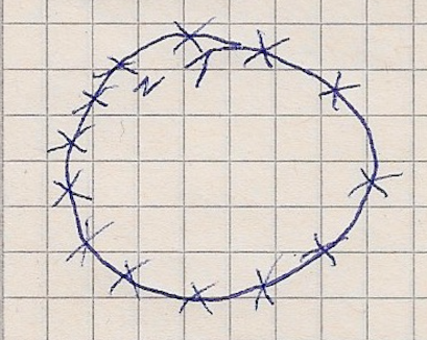
\includegraphics[width = \textwidth]{Zeichnungen/36.pdf}
  \caption{das N-te Teilchen wechselwirkt mit dem Ersten.}
  %\label{fig:Bild}
\end{figure}

\begin{align}
    H &= \sum_j H_j \quad ,\hat\sigma_j=2\hat S_{j,z}\\
    \hat H_j &= -J\hat\sigma_j \hat\sigma_{j+1}\\
    \text{Ising-Basis:} &\Ket{\sigma_1,\sigma_2,...,\sigma_j,...\sigma_N} \quad \sigma_j=\pm1\\
    \hat\sigma_j\Ket{\sigma_1,...,\sigma_j,...\sigma_N}&=\hat\sigma_i\Ket{\sigma_1,...,\sigma_j,...\sigma_N}\\
    [H_i, H_j] = 0  \qquad \Rightarrow \e^{-\beta \hat H} &= \prod_{j=1}^N \e^{-\beta \hat{H}_j} \\
    \text{Zustandssumme: } Z(T,N,h)&= \Tr\left[\e^{-\beta\hat H}\right]=\Tr\left[\prod_j \e^{-\beta H_j}\right]\\
    &=\Tr\left[\e^{-\beta\hat H_1}....\e^{-\beta\hat H_{j-1}}\underarrow{ }{\hat 1 = \sum_{\sigma_j}\Ket{\sigma_j}
    \Bra{\sigma}\hspace{2.5cm}} \e^{-\beta\hat H_{j}}\underarrow{ }{\hspace{2.5cm}\hat 1 = \sum_{\sigma_j+1}\Ket{\sigma_j}}\e^{-\beta\hat H_{j+1}}
    \e^{-\beta\hat H_{N}}\right]\\
    \text{Transfermatrix: } P_{\sigma_j \sigma_{j+1}} &= \Bra{\sigma_j} \e^{-\beta \hat{H}_j} \Ket{\sigma_{j+1}} = \e^{-\beta(-J \sigma_j \sigma_{j+1} +\frac{h}{2}(\sigma_j + \sigma_{j+1})} \\
\end{align}
\begin{align}
    2 \times 2-\text{Matrix:} \quad P &=
    \begin{pmatrix}
        \e^{\beta(J-h)} & \e^{-\beta J} \\
        \e^{-\beta J} & \e^{\beta(J+h)} \\
    \end{pmatrix}\\
    Z(T,N,h)&=\Tr[P^N]=\lambda_+^N+\lambda_-^N \\
    \lambda_\pm &\quad \text{Eigenwerte von } \tensor{P}\\
    \tensor P &= \tensor U \underbrace{
    \begin{pmatrix}
        \lambda_+ & 0\\
        0   & \lambda_-\\
    \end{pmatrix}}_{\tensor D_p}\tensor U ^{-1} \\
    \tensor P^N &= \left[ \tensor U \tensor D_P \tensor U^-\right]^N = \tensor U \tensor D_P^N \tensor U^{-1}\\
    x&=\e^{\beta J}, \quad y=\e^{-\beta h} \\
    O&=\lvert \tensor P -\lambda \tensor 1 \rvert=
    \begin{vmatrix}
        xy-\lambda & \frac{1}{x} \\
        \frac{1}{x}  & \frac{x}{y}-\lambda\\
    \end{vmatrix} \\
    &=(xy-\lambda)(\frac{x}{y}-\lambda)-\frac{1}{x^2}=\lambda^2-\lambda x(\underarrow{y}{2\cosh(\beta h)}+\frac1y)+x^2-\frac{y}{x^2}=0\\
\end{align}
\begin{align}
    y + \frac{1}{y} &= \e^{-\beta H} + \e^{\beta H} = 2 \cosh(\beta h) \\
    x^2 - \frac{1}{x^2} &= \e^{2 \beta J} - \e^{2 \beta J} = \sinh(2 \beta J) \\
    \lambda_{\pm} &= x \cosh(\beta h) \pm \sqrt{x^2 \cosh^2(\beta h) - 2\sinh(2\beta J) } \\
    &= \e^{\beta J} \left[\cosh(\beta h) \pm \sqrt{\cosh^2(\beta h) - 2\e^{-2\beta J} \sinh(2\beta J))} \right] \\
    \lambda_{+} &> \lambda_{-} \\
    \frac{1}{N}\Phi(T,N,h)&=-\frac{\kB T}{N} \ln(\underbrace{\lambda_+^N+\lambda_-^N}_{\lambda_+^N\left(1+\left(\frac{\lambda_-}{\lambda_+}\right)^N\right)})\\
    &=-\kB T\ln\lambda_+ -\frac{\kB T}{N} \ln\left(1+\underbrace{\left(\frac{\lambda_-}{\lambda_+}\right)^N}_{<1,\to 0,N\to \infty}\right)\\
    \lim_{N\to \infty} \frac 1N \Phi (T, N, h) &= -\kB T \ln(\lambda_+)\\
    &= -J - \kB T \ln\left[\cosh(\beta h) + \sqrt{\cosh^2(\beta h) - 2 \e^{-2\beta J} \sinh(2\beta J) }\right]\\
    m &= \frac{M}{N} = - \frac{1}{N} \pdif{\Phi}{h}[T, N] \\
    &= \cancel{\kB T} \frac{\cancel{\beta} \sinh(\beta h)}{\cancel{\cosh(\beta h) + \sqrt{...}}} \left[\underbrace{1+\frac{1}{\cancel{2}} \frac{\cancel{2} \cosh(\beta h)}{\sqrt{...}}}_{\cancel{\frac{\sqrt{...}+\cosh(\beta h)}{\sqrt{...}}}} \right] \\
    &= \frac{\sinh(\beta h)}{\sqrt{\cosh^2(\beta h)  - 2 \e^{-2 \beta J} \sinh(2 \beta J)}} \\
    \lim_{h\to 0}m(h) &= 0 \Rightarrow m\approx h \Rightarrow m=\chi h \qquad (\chi:\text{mag. Suszeptibilität})\\
    &\text{Magnetische Phase: } \lim{h \to 0} m(h) = m_0 \pm 0 \\&(\text{nicht im $1D$ Ising-Modell bei $T>0$})\\
    \chi&=\pdif{m}{h}[h=0]
\intertext{2 Strategien in der Theorie der Phasenübergänge}
\end{align}

\begin{enumerate}
    \item Symmetriebrechung durch ein externes Feld $(h)$
    \item Berechne $\chi(h=0)$
\end{enumerate}

\begin{align}
    \chi(T)\biggr\vert_{h\to 0}&=\pdif{m}{h}[h\to 0] =\beta\left[\frac{\cosh(\beta h)}{\sqrt{...}}-\frac12 \frac{\sinh(\beta h)^2(\to 0)}{\sqrt{..}^3}\right]\biggr\vert_{h\to 0} \\
    &= \beta \frac{1}{\sqrt{\cancel{1} - \cancel{2} \underbrace{\e^{-2\beta J} \frac{1}{\cancel{2}} (\e^{2 \beta J} -\e^{-2\beta J)}}_{1-\e^{-4\beta J}}}} = \beta \e^{2 \beta J} \\
\intertext{1. Fall: nicht wechselwirkende Spins: $J=0$}
    \chi(T)&=\frac{1}{\beta} =\frac{1}{\kB T} \propto \frac{1}{T} \quad \text{Curie-Gesetz für ein freies mag. Moment}\\
    \chi(T)&=\frac{1}{\kB T}\e^{2\beta J}\text{steigt stärker an als das Curie-Gesetz für $J\neq 0$} \\
    \lim_{T \to \infty} &\to \infty \\
    \text{Entropie pro Gitterplatz:} &\quad \frac{S}{N}=-\frac{1}{N}\pdif{}{T}\Phi \text{ stetig}\\
    \text{Spezifische Wärme:} &\quad  C_V = T \pdif{S}{T} \text{stetig für $T>0$}\\
\intertext{2D-Ising-Modell: kritische Temperatur $ T_C > 0; T_C \approx J$}
\end{align}

\subsection{Theorie des mittleren Feldes}
\begin{align}
    H &= -J \sum_{<i,j>} \vec{S}_i \vec{S}_j \qquad \text{Heisenberg-Modell}\\
    &=J\sum_i \vec S(-J)\underbrace{\sum_{<j,\text{max}>} \vec{S}_j}_{\vec B_i^{\text{eff}}}
\end{align}
\begin{figure}[H]
  \centering
  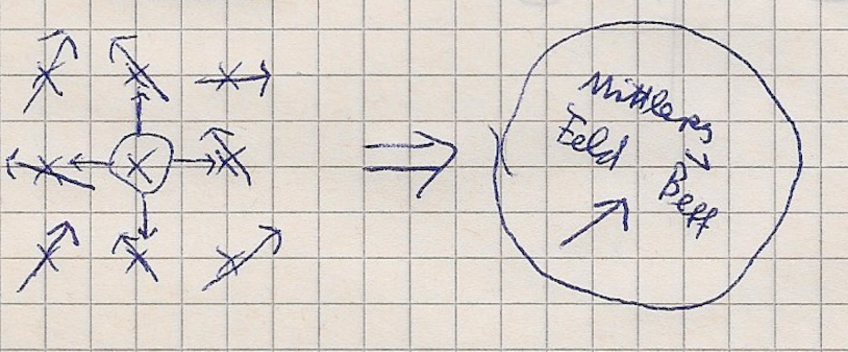
\includegraphics[width = \textwidth]{Zeichnungen/37.pdf}
  \caption{Spins koppeln nur mit nächsten Nachbarn.}
  %\label{fig:Bild}
\end{figure}
\begin{align}
    F[\hat \rho] &= \Braket{\hat H} - T S[\hat \rho] = \Tr[\rho \hat H] + \kB T \Tr[\hat \rho \ln \hat \rho]\\
\intertext{ist für das Heisenberg Modell nicht exakt lösbar für $D>1$ }
    \hat\rho_\text{th} &= \frac{\e^{\beta \hat H}}{Z}; \qquad Z = \Tr [\e^{-\beta \hat H}]\\
    F[\hat \rho] &\geq F[\hat \rho_\text{th}]\\
\intertext{Näherung:}
    \rho_\text{th}\to \hat \rho_\text{trial}(\lambda_1,\lambda_2,..\lambda_N...)
\end{align}
\begin{enumerate}
    \item Einschränkung im Raum der Dichteoperatoren
    \item $F[\rho_\text{trial}(\lambda_i)] \geq F[\rho_\text{th}]$ \\
    Variationsansatz: \\
    \begin{align}
        \pdif{F}{\lambda_i} = 0 \ \forall \lambda_i
    \end{align}
\end{enumerate}
Frage: Wie wählen wir $\hat \rho_\text{trial}$?
\begin{align}
    \text{Antwort: } \rho_\text{trial} &= \frac{\e^{-\beta\hat H_\text{eff}}}{Z_\text{MF}}, \quad Z_\text{MF} = \Tr\left[\e^{-\beta\hat H_\text{eff}}\right]
    H_\text{eff}=-\sum_j \vec S_i \vec X_i\\
    [\vec X_i]: &\qquad \text{Energie, klassischer Vektor}
\end{align}

\begin{figure}[H]
  \centering
  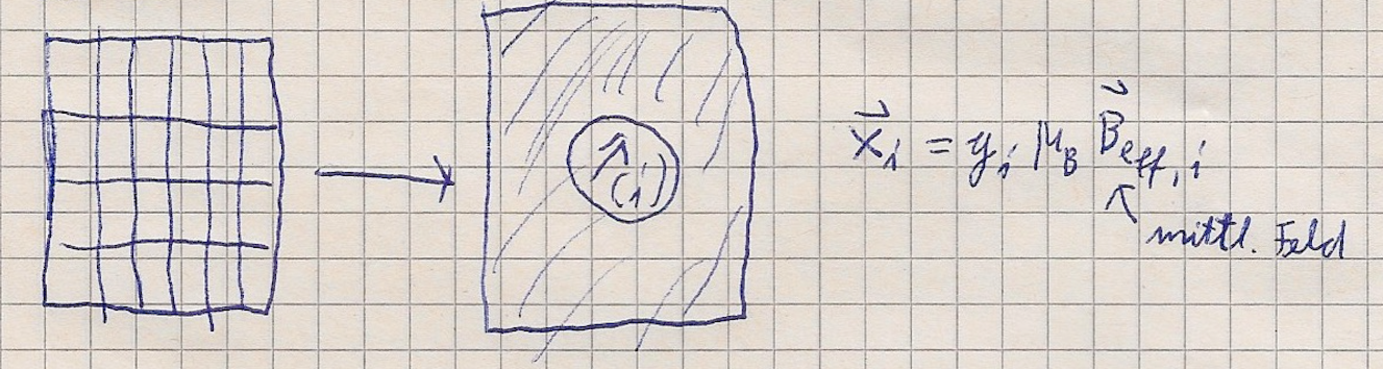
\includegraphics[width = \textwidth]{Zeichnungen/38.pdf}
  \caption{Spin in einem Magnetfeld $\vec x_i$.}
  %\label{fig:Bild}
\end{figure}
\begin{align}
    F[\hat \rho_\text{MF}(\{\vec X_i\})]&=F(\{\vec X_i\})=\Tr[\rho_\text{MF} \hat H]+\kB T \Tr[\rho_\text{MF}(-\beta \hat H_\text{eff} -\ln Z_\text{MF})]\\
    &=\Tr[\rho_\text{MF}(\underarrow{H-H_\text{eff}}{\text{Korrekturterm}\ \Braket{\Delta H}})]-\frac{1}{\beta} \ln Z_\text{MF}
\intertext{Zustandssumme:}
    Z_\text{MF}&=\Tr[\e^{-\beta H_\text{eff}}]=\Tr[\e^{\sum_i \beta \vec S_i \vec X_i}]=\prod_{i=1}^N \Tr[\e^{\beta \vec S_i \vec X_i}]=\prod_i Z_i\\
    \Tr\left[\hat \rho_\text{MF} \hat H_\text{eff}\right] &= - \sum_j \Tr\left[\rho_\text{MF}\vec S_i \vec X_i\right] = -\sum_j \Braket{\vec S_j} \vec X_j\\
    \Tr\left[ \rho_\text{MF} \hat H \right] &= - J \sum_{ \Braket{j, i}} \Tr[\rho_\text{MF} \vec S_i \vec S_j]
    = - J \sum_{\Braket{j, i}} \Braket{\vec S_i} \Braket{S_j}
\end{align}

\begin{align}
    F(\{\vec{x}_i\}) &= - \sum_{i} \Braket{\vec{S}_n} \left( \left(\sum_{j \in NN(n)} J \Braket{\vec{S}_j} \right)  - \vec{x}_n \right) - \frac1{\beta} \ln(Z_\text{MF}) \\
    0 &= \pdif{F}{X_{i,\underarrow{\alpha}{\alpha=x,y,z}}}
    = \cancel{\Braket{S_{i,\alpha}}} - \sum_n \vec{X}_n \pdif{\Braket{\vec S_n }}{X_{i,\alpha}} - J
    \underbrace{
        \pdif{}{X_{i,\alpha}} \left(\sum_{\Braket{n,m}} \Braket{\vec S_n} \Braket{\vec S_m}\right)
    }_{
        \underbrace{
            \sum_{\Braket{n,m}} \pdif{\Braket{\vec S_n}} {x_{i,\alpha}} \Braket{\vec S_m} + \Braket{\vec S_n} \pdif{\Braket{\vec S_m}}{x_{i,\alpha}}
        }_{
            2\sum_{\Braket{n,m}} \Braket{S_n} \pdif{\Braket{\vec S_m}}{x_{i,\alpha}}
        }
    } \\
    &-\frac{1}{\cancel{\beta}}\underbrace{
        \cancel{\frac{1}{Z_\text{MF}}\cancel{\beta} \Tr[S_{i,\alpha}\e^{\beta\vec S_{i}\vec X_{i} }]\prod_{n\neq i} Z_i}
    }_{
        \Braket{\hat S_{i,\alpha}}
    }
    \\&= \sum_n \left(\vec X_n - 2 J \sum_{m \in NN(n)} \Braket{\vec S_m}\right) \underarrow{\pdif{\Braket{\vec S_n}}{X_{i, \alpha}}}{\neq 0} = 0 \\
    \Rightarrow \Aboxed{\vec X_n &= 2 J \sum_{m \in NN(n)} \Braket{\vec S_m}} \qquad \text{MF Selbstkonsistenzgleichung}\\
    \vec X_n &= 0 \Rightarrow \Braket{\vec S_j} = 0 \quad \text{ist immer eine Lösung }
\intertext{paramagnetische Phase}
\end{align}
Hier: $J > $: Ferromagnetismus
\begin{itemize}
    \item Alle Spins richten sich in z-Richtung aus
    \item Translationsinvariante Lösung
\end{itemize}

\begin{align}
    \vec{x}_n \to \vec{x} &\neq x \vec e_z\\
    \text{SCG: }\ x &=2 p J\Braket{S_z}  \quad; p = \text{\# nächste Nachbarn} = 2d\\
    Z_i &= Z=\Tr[\e^{\beta S_z x}]=\sum_{m=-L}^L \e^{\beta m x} \\
    &= \e^{\beta L x} \sum_{m=0}^{2 L} e^{-\beta m x}=\e^{\beta L x} \frac{\e^{-\beta(2L+1)x}-1}{\e^{-\beta x}-1}\\
    &= \frac{\e^{-\beta (L+1)x} - \e^{\cancel{-}\beta L x}}{\e^{-\beta x} - 1 } \frac{\e^{\beta \frac L2 x}}{\e^{\beta \frac L2 x}} = \frac{\sinh \left(\left(L + \frac12\right)\beta x\right)}{\sinh \left(\frac L2 \beta x\right)}\\
    \Braket{S_z} &= \frac 1Z \Tr\left[\hat S_z \e^{\beta S_z x}\right] = \frac 1\beta \pdif{}{x} (\ln(Z)) \\
    &= (L + \frac12) \coth\left(\beta \left(L + \frac12\right)x\right) - \frac L2 \coth\left( \frac{\beta x}{2}\right)\\
\intertext{wir verwenden die Identität $\equiv L B_L(\beta L x)$}
    \pdif{}{x}\ln(\sinh(\alpha x)) &= \alpha \frac{\cosh(\alpha x)}{\sinh(\alpha x)}
\intertext{Brillouin-Funktion}
    B_L(x)&=\frac{2L+1}{2L} \coth(\frac{2L+1}{2L}x)-\frac{1}{2L}\coth(\frac{1}{2L}x)
\intertext{Spin $\frac12$}
    B_\frac12(x) &= 2 \coth(2 x) - \coth(x)
    = 2\underbrace{\frac{\e^{2x}+\e^{-2x}}{\e^{2x}-\e^{-2x}}}_{(\e^{x-\e^{-x}})(\e^{x}+\e^{-x})} -\frac{(\e^{x}+\e^{-x})^2}{(\e^{x}-\e^{-x})(\e^{x}+\e^{-x})} \\
    &= \frac{\overbrace{\cancel{2} (\e^{2x} + \e^{-2x}) - (\cancel{\e^{2x} + \e^{-2x}} + 2)}^{4 \sinh^2(x)}}{(+) (-)} \\
    &=\frac{\cancel{4}\sinh^{\cancel{2}}(x)}{\cancel{4}\cancel{\sinh(x)}\cosh(x)}=\tanh{x}\\
    \Aboxed{x &=  pJ \tanh(\beta \frac x2)}
\end{align}

\begin{align}
    \hat \rho_\text{MF} &= \frac 1Z_\text{MF} \e^{-\beta \hat H_\text{eff}}; \qquad H_\text{eff} = -\sum_j \vec S_j \vec X_j\\
    \vec X_j &= g \mu_B \vec B_j^\text{eff}\\
    \Braket{S_Z} &= \frac LL \left(L + \frac12 \right) \coth \left(\beta \left(l + \frac12 \right) X \frac LL \right) - \frac12 \frac LL \coth \left(\beta \frac x2 \frac LL \right)\\
    &= L B_L(\beta Lx)\\
    \Aboxed{X &= 2pJ\Braket{S_z}} \quad \text{für} \quad X_i = X\\
    B_L{x} &= \frac{2L+1}{2L} \coth(\frac{2L+1}{2L} x) - \frac{1}{2L}\coth(\frac{x}{2L}) \\
\end{align}
%Bild 39 caption:
\begin{figure}[H]
  \centering
  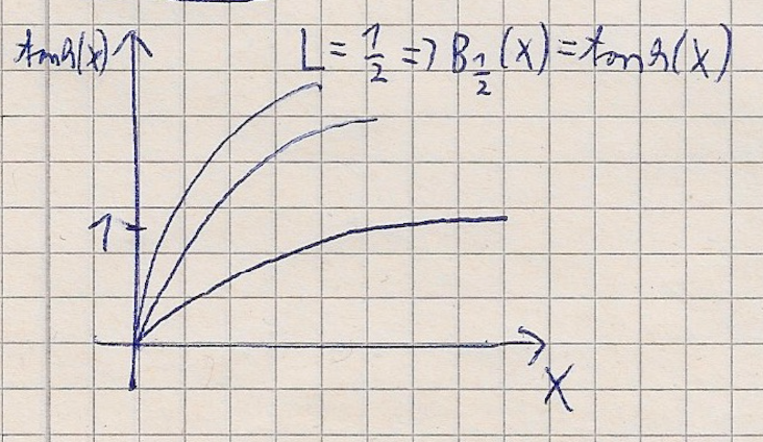
\includegraphics[width = \textwidth]{Zeichnungen/39.pdf}
  \caption{.}
  %\label{fig:Bild}
\end{figure}
%Bild 40 caption:
\begin{figure}[H]
  \centering
  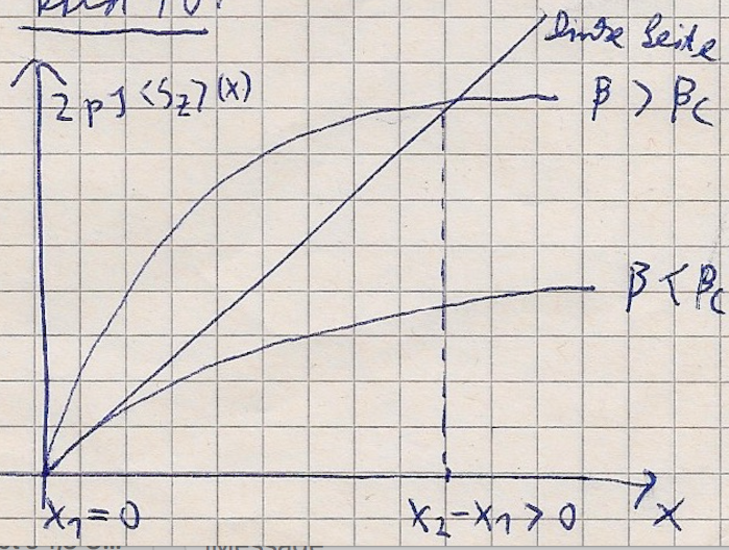
\includegraphics[width = \textwidth]{Zeichnungen/40.pdf}
  \caption{.}
  %\label{fig:Bild}
\end{figure}
\begin{enumerate}[i]
    \item Paramagnetische Phase (PM)
    \begin{itemize}
        \item $\beta$ < $\beta_c$ \quad $T>T_c$
        \item $\Braket{S_z} = 0$ \quad $X=0$
    \end{itemize}
    \item Ferromagnetische Phase (FM)
    \begin{itemize}
        \item $\beta$ > $\beta_c$ \quad $T<T_c$
        \item $\Braket{S_z} > 0$ \quad $X>0$
    \end{itemize}
\end{enumerate}

\begin{align}
    \intertext{Spinsuszeptibilität (PM):}
    \increment H &= H_1 = - \sum_j \vec{S}_j (g \mu_\text{B} \vec{B}_\text{ex}) = - \sum_j \vec{S}_j \vec{x}_\text{ex} \\
    \text{mit: } \quad \alpha, \beta &= x, y, z\\
    X_{\alpha, \beta} &= \pdif{M_\alpha}{B_\beta} = \pdif{(g \mu_B \Braket{S_\alpha})}{B_\beta} \frac{(g \mu_B)}{(g \mu_B)} = (g \mu_B)^2 \pdif{\Braket{S_\alpha}}{X_\alpha} \delta_{\alpha, \beta}\\
    \chi_{\alpha \beta} &= \delta_{\alpha \beta} (g \mu_\text{B})^2 \beta L^2 B_L'(\beta L x)\vert_{x \to 0} \\
\intertext{Taylor-Entwicklung}
    \coth{x} &= \frac{1}{x} + \frac{x}{3} - \frac{x^3}{45} + \mathcal O(x^5) \\
    B_L(x) &= ... = \frac{L+1}{3L} x - \frac{x^3}{45} \frac{(2L+1)^4-1}{(2L)^4} + \mathcal O(x^5) \\
    \Chi_{\alpha, \beta} &= \delta_{\alpha, \beta} (g \mu_B )^2 \beta L^{\cancel{2}} \frac{(L + 1)}{3\cancel{L}} = \delta_{\alpha, \beta} \underbrace{(g\mu_B)^2 \frac{L(L+1)}{3} \frac{1}{\kB T}}_{\text{Curie-Gesetz}}
\end{align}

\paragraph{Selbstkonsistente Lösung der Mean-Field-Gleichung:}


\begin{align}
    \Braket{S_Z} &= L B_L (\beta L x ) \stackrel{x \to 0}{\approx} \cancel{L} \frac{(L + 1)}{3 \cancel{L}} (\beta L X) + \mathcal O(x^3)\\
    &\text{Mean-Field-Gl.} \quad X \to 0 \\
    X &= 2P J \Braket{S_z} \approx 2P J \frac{L(L+1)}{3} \beta X\\
    \Rightarrow \Aboxed{\kB T_\text{C} &= 2pJ \frac{L(l+1)}{3}} \\
    x &= 0 \qquad \text{für: } \quad T_C < T\\
    x &\neq 0 \qquad \text{für: } \quad T < T_C
\end{align}

Frage:
\begin{itemize}
    \item $x>0$: Thermodynamisch stabil, $F(x) < F(0)$?
    \item Analytische Form von $X(T)$
\end{itemize}


\begin{align}
    F(x) &= - \sum_j \Braket{\vec S_j} \sum_{m \in NN(j)} J \Braket{\vec S_m} - \underarrow{\vec X_j}{X \vec e_z}) - \frac 1\beta \ln(Z_\text{AF}) \\
    &(NN(j) = \text{\enquote{nearest neighbours of $j$}})\\
    &= -N \frac{X}{2pJ} \left( \cancel{p} \frac{\cancel{J} X}{2 \cancel{pJ}} - X \right) - N \ln \left(\frac{\sinh((L+\frac{1}{2}) \beta x)}{\sinh(\beta \frac{x}{2})} \right)  \qquad \Aboxed{ \Braket{S_z} = \frac{X}{2PJ}} \\
    &= N \left[ \frac{X^2}{4 p J} - \frac 1\beta \ln(...)\right]
\end{align}

\begin{align}
\intertext{Nebenrechnung}
    \sinh(y) &= y + \frac{y^3}{3!} + \mathcal O(y^5)\\
    \ln(1 + y) &= y - \frac{y^2}{2} + \mathcal O(y^3)
\end{align}

\begin{align}
    \ln \left( \frac{\sinh(ax)}{\sinh(bx)} \right) &\approx \ln \left( \frac{ ax + \frac{1}{6} (ax)^3 +...}{ bx + \frac{1}{6} (bx)^3 +...} \right)\\
    &= \ln \left(\frac ab \frac{1 + \frac16 (ax)^2 ...}{1 + \frac16(bx)^2 ...} \right) = \ln \left( \frac{a}{b} \right) + \left(\frac{(ax)^2}{6} - \frac{(bx)^2}{6} \right) + \mathcal O(x^4) \\
    &= \ln \left(\frac ab \right) + \frac{x^2}{6} (a^2 - b^2) + \mathcal O(x^4)\\
    \text{mit:} \quad a &= \beta\left(L + \frac12 \right) \quad b = \frac \beta2\\
    \frac{F(x)}{N} &\approx \frac{X^2}{4pJ} - \frac1{\cancel{\beta}} \left[ \ln (2L+1) + \frac{x^2}{6} \frac{\beta^{\cancel{2}}}{\cancel{4}} [\underbrace{(2L+1)^2-1}_{2L(2L+1) = \cancel{4}L(L+1)}]+...\right] \\
    &\approx  T \underbrace{\kB  \ln (2L + 1)}_{\text{Entropie pro Spin}} + \frac{X^2}{4 pJ} - \beta \frac{L(L + 1)}{6} x^2\\
    F &= U - TS
\end{align}

\begin{align}
    \kB T_\text{C} &= 2p J \frac{L (L+1)}{3}\\
    \beta_\text{C} &= \frac{3}{2pJ L(L+1)} \Rightarrow \frac{1}{4pJ} = \frac{L(L+1)}{6} \beta_C\\
    \frac{F(x)}{N} &\cong -\kB T \ln (2L+1) + \underbrace{x^2\left(\beta_\text{C} \frac{L(L+1)}{6} - \beta \frac{L(L+1)}{6} \right)}_{ x^2 \frac{L(L+1)}{6} \beta_\text{C}\underbrace{\left(1- \frac{\beta}{\beta_C} \right)}_{1-\frac{T_\text{C}}{T}}} \\
    \text{Für: } T < T_C \quad &\hat = \quad \beta > \beta_C\\
    \text{gilt: } (1- \frac{\beta}{\beta_C}) &< 0\\
    \Rightarrow F(x) - F(0) &< 0 \quad \text{für} \quad T < T_\text{C} \\
\intertext{$\Rightarrow$ thermodynamisch stabil} \\
    (ii) \to X(T) &= ? \\
    \Braket{S_z} &= \frac{L(L+1)}{J} \beta X \left( 1 - \underarrow{\frac{L^2 + L + \frac12 }{15}}{Y^2} (\beta x)^2 + \cdots \right)\\
    X &= \underbrace{2pJ \frac{L(L+1)}{3}}_{\frac{1}{\beta_\text{C}}} \beta X (1 - \gamma ^2 (\beta x)^2) \\
    \cancel{X} &\approx \frac{\beta}{\beta_C} \cancel{X} ( 1 - \gamma^2 (\beta X )^2 )\\
    \frac{\beta_\text{C}}{\beta} &= (1 - \gamma^2 (\beta X)^2)\\
    \gamma^2 (\beta x)^2 &= 1 - \frac{\beta_\text{C}}{\beta} = 1 - \frac{T}{T_\text{C}} = \frac{T_\text{C} -T}{T_\text{C}} = t \quad \text{reduzierte Temperatur} \\
    X &= \frac{\kB T_\text{C}}{\gamma} t^\frac12  = A t^\beta\\
\intertext{$\beta$: kritischer Exponent des Ordnungsparameters \rightarrow MF-Theorie $\beta = \frac{1}{2}$}
\end{align}
%Bild41 caption:
\begin{figure}[H]
  \centering
  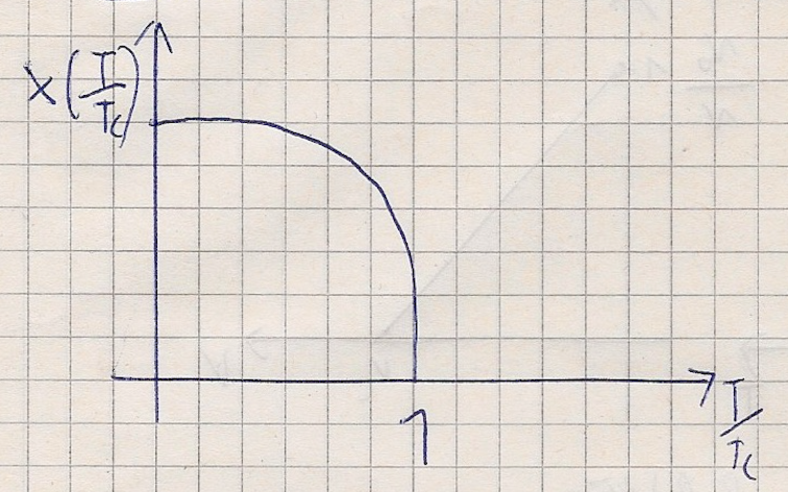
\includegraphics[width = \textwidth]{Zeichnungen/41.pdf}
  \caption{.}
  %\label{fig:Bild}
\end{figure}

\subsection{Landau-Theorie der Phasenübergänge}
Räumliche  Mittelung:
%Bild42 caption: Mittelung
\begin{figure}[H]
  \centering
  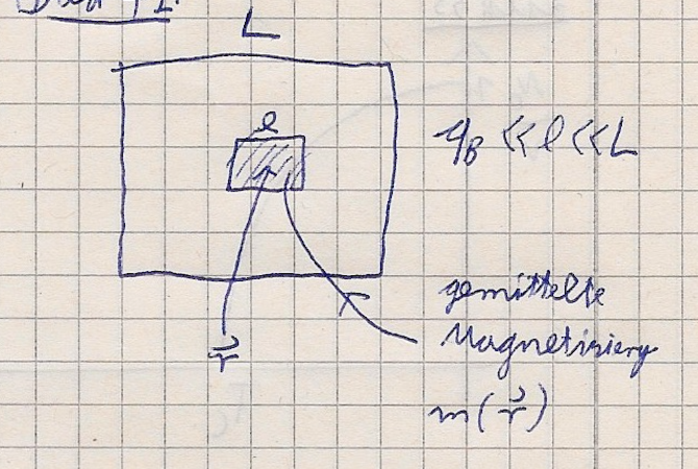
\includegraphics[width = \textwidth]{Zeichnungen/42.pdf}
  \caption{Mittelung.}
  %\label{fig:Bild}
\end{figure}
Allgmeiner: $m(\vec r)$
\begin{align}
    l:\text{mikroskopisch groß aber makroskopisch klein}
\intertext{Vereinfachung}
\end{align}
 \begin{enumerate}
    \item Vernachlässigung von Räumfluktuationen:$m(\vec{r},T) \to m(T)$
    \item M sei statisch und verschwindet bei $T=T_c$
        \begin{align}
            m(T>T_c) &= 0\\
            m(T<T_c) &\neq 0
        \end{align}
    \item $F(m,T)$ wird als Taylorreihe in m entwickelt
\end{enumerate}
\begin{align}
    \intertext{nahe $T_c$ gilt:}
    F(m,H) &\tilde{=} T_0+\frac 12 r_0(T)m^2+U_0 m^4 - m \underarrow{H}{\text{externes Magnetfeld}}
\intertext{Für $H=0$}
%Bild43 caption: für H=0
\end{align}

\begin{figure}[H]
  \centering
  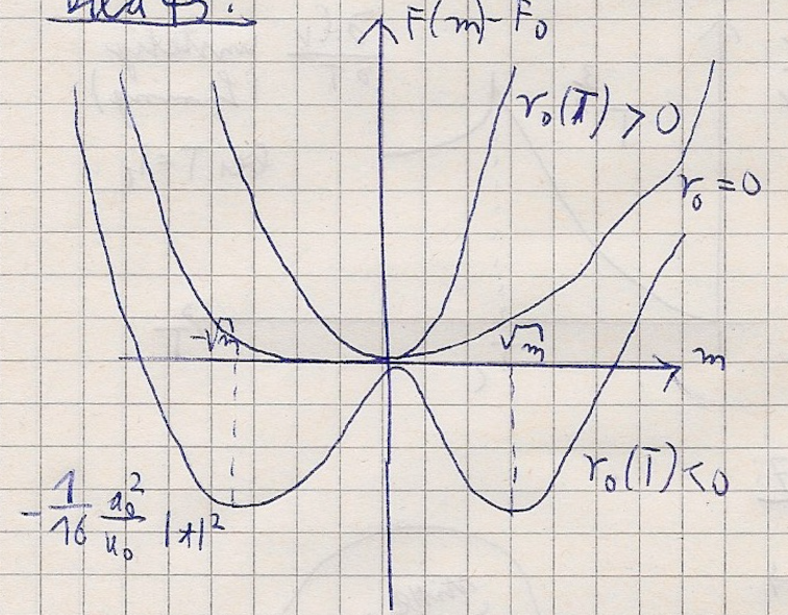
\includegraphics[width = \textwidth]{Zeichnungen/43.pdf}
  \caption{für $H=0$.}
  %\label{fig:Bild}
\end{figure}

\begin{align}
\intertext{Minimierung der Freien Energie}
    \pdif{F}{m}&= r_0(T) m+4 U_0 m^3 -H=0
\intertext{Für $H=0 \Rightarrow$ zwei Lösungen}
\end{align}
\begin{itemize}
    \item triviale Lösung $m=0$
    \item \begin{align}
            r_0(T) + 4 k_0 m^2 &= 0\\
            m^2 = - \frac{r_0(T)}{4 k_0} \Rightarrow m_\pm &= \pm \sqrt{\frac{|r_0(T)|}{4k_0}}
          \end{align}
\end{itemize}
\begin{align}
\intertext{Entwicklung von $r(T)$ um $T_c$}
    r_0(T) &\approx \underbrace{r_0(T_c)}_{=0}+\overline{a}_0(T-T_c)= \underline{\overline{a}}_0 T_c  \frac{T-T_c}{T_c}=a_0 t\\
    t &= \frac{T-T_c}{T_c} \text{reduzierte Temperatur}\\
    \Rightarrow \bar{M} &= \sqrt{- \frac{a_0}{4 k_0} t} \underarrow{=}{t<0} \sqrt{\frac{a_0}{4 k_0} |t|} \propto |t|^{frac12} = |t|^{\beta}
\intertext{kritischer Exponent $\beta =\frac 12$}
    F(\overline{m})-F_0&\underarrow{=}{t<0} \frac 12 a_0 t \frac{a_0}{4U_0}\lvert t\rvert+\cancel{U_0}\frac{a_0^2}{16 U_0^{\cancel{2}}}\lvert t\rvert^2=-\frac{1}{16} \frac{a_0^2}{U_0}\lvert t\rvert^2 < 0\\
    t|t| &= -|t|^2\\
\intertext{Suszeptibilität}
    \Chi &= \pdif{m}{H}[H\to 0]\\
    r_0(T) \underbrace{\pdif{m}{H}}_{\Chi} + 4k_0 3 m^2 \underbrace{\pdif{m}{H}}_{\Chi} -1 &= 0\\
    \Rightarrow \Aboxed{\chi &= \frac{1}{r_0(T) + 12 k_0 m^2}} \quad \text{mit } m = \overline m
\end{align}
\begin{enumerate}
    \item   \begin{align}
            T>T_c \Rightarrow \overline{m}=0\\
            \Chi=\frac{1}{r_0(T)}=\frac{1}{a_0} t^{-1}=\frac{1}{a_0}\lvert t\rvert^{-1}
            \end{align}
            $\chi$ divergiert an $T_c$
            \begin{align}
                \Chi \propto \lvert t \rvert^{-\gamma}\Rightarrow \gamma = 1
            \end{align}
    \item $T< T_C (t < 0)$
            \begin{align}
                \text{Nenner: } r_0 + 12 U_0 \left(-\frac{r_0}{4 k_0}\right) &= - 2r_0 = - 2a_0 t = 2 a_0 |t|\\
                \chi &= \frac{1}{2a_0 \lvert t \rvert} \propto \lvert t\rvert^{-1}\\
            \intertext{Phasenübergang 2. Ordnung (kontinuierlicher Phasenübergang)}
            \intertext{Spontane Symmetrie Berechung}
                \text{Spezialfall: } r_0(T) &= 0\\
                4 k_0 m^3 - H &= 0\\
                m = \left(\frac{1}{4 k_0}\right)^{\frac13} H^\frac13 \propto H^\frac1\delta \Rightarrow \delta &= 3
            \end{align}
\end{enumerate}
Spezifische Wärme
\begin{align}
    C_V &= T \pdif{S}{T}\\
    \Delta C_v &= T\pdif{\Delta S}{T}\\
    \Delta S &= - \pdif{\Delta F}{T}=\pdif{}{T} \left(\frac{a_0^2}{16U_0} \frac{(T-T_c)^2}{T_c^2} \right)\\
    &=\frac{a_0^2}{8 U_0} \frac{1}{T_c^2}(T-T_c)
\intertext{$\Rightarrow S$  ist an $T_c$ stetig, da $\Delta S(T_c)=0$}
    T\pdif{\Delta S}{T} &= \frac{a_0^2}{8 U_0}\frac{T}{T_c}>0
\end{align}
%Bild 44 caption: $C_V$ hat einen Sprung bei $T_C$
\begin{figure}[H]
  \centering
  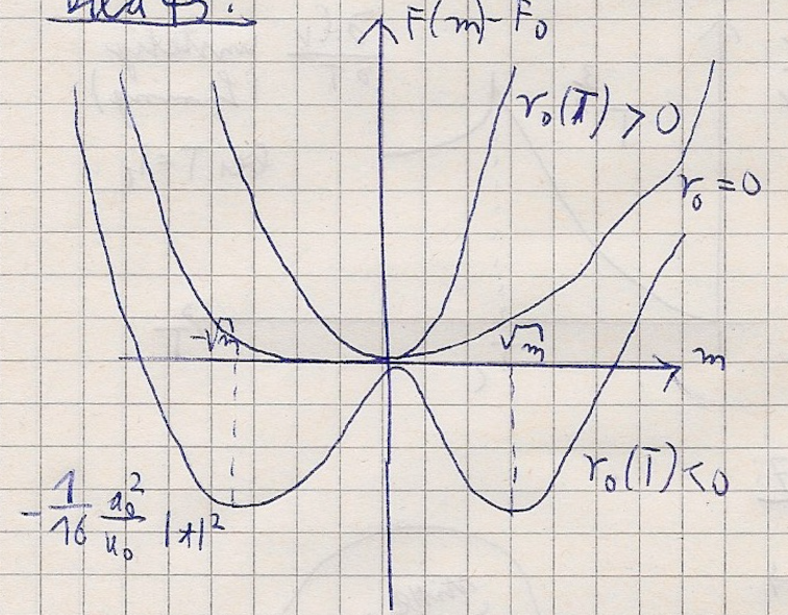
\includegraphics[width = \textwidth]{Zeichnungen/43.pdf}
  \caption{$C_V$ hat einen Sprung bei $T_C$.}
  %\label{fig:Bild}
\end{figure}
\begin{align}
    C_v\propto &\lvert t\rvert^{-\alpha}\\
    \text{Hier } \alpha &=0 \lvert\text{keine Divergenz um $C_v(T\to T_c)$}\\
\intertext{Ausblick:}
    F[m(\vec{r})] &= \int \dif^d r \left(\frac 12 r_0(T)m(\vec r)^2+U_0 m(\vec r)^2+\frac 12 \lvert \nabla m \rvert^2-hm(\vec) \right)\\
    F &= -\frac 1\beta \ln(Z) \rightarrow Z = \int D[m] \e^{-\beta F [m(r)]}\\
    Z &=\Tr[e^{-\beta H}]
\end{align}

\subsection{Das Theorem von Mermin und Wagner (1966)}

In $1D$ und $2D$ kann es im isotropen Heisenbergmodell keine spontane Magnetisierung geben. 2($T_C > 0$ nicht möglich.)
Verallgemeinerung auf andere Probleme mit kon. Symmetriebrechung, z.B. Supraleitung um Kristallisation.
\begin{align}
    \intertext{Thermodynamischer Limes}
    \overline{O}=\lim_{V\to\infty,N\to \infty} \frac{1}{V} \Braket{\hat O},   \quad \quad \text{$\hat O$ extensiv}
\end{align}

\paragraph{Theorem von Mermin und Wagner}
In 1D und 2D gibt es keine spontane Symmetriebrechung einer \emph{kontinuierlichen} Symmetrie.
Sei $\hat\Gamma_s^i$ ein Generator der Symmetrietrafo (Beispiel $\vec{S}(\vec{L})$ erzeugen eine Drehung)
\begin{align}
    [\hat H,\hat \Gamma_S^i]&=0\\
\intertext{falls: }
    \hat C_i&=[\hat A ,\hat \Gamma] \qquad (\text{Beispiel }\ S_z=i\hbar[S_x,S_y])
\intertext{dann gilt:}
    \Braket{\hat C_i} &= \Braket{[A, \Gamma_S^i]} = \Tr [\underarrow{\hat \rho}{\rho = \frac{\e^{-\beta H}}{Z} \Rightarrow [\rho, \Gamma_S^i = 0]} (\hat A \Gamma_s^i - \Gamma_S^i \hat A)] = 0
\intertext{Wir brechen die Symmetrie explizit:}
    H_g &= H-g\hat V, \qquad [\hat V,\Gamma_s]\neq 0\\
    \overline{O}_q&=\lim_{g \to 0}\lim_{\substack{V\to 0 \\ (N\to 0)}} \Tr\left[ \frac{\e^{-\beta H_g}}{Z_q} \hat O\right]
\intertext{Heisenbergmodell}
    H_b&=\underbrace{-\sum_{ij} J_{ij} \vec{S}_i \vec{S}_j}_{H} -b\sum_j S_j^z \e^{-i\vec{\mathcal K} \vec R_j}
\intertext{Wähle $\vec \mathcal K$:}
    \text{Ferromagnetisch: } \vec \mathcal K &= 0\\
    \text{Anti-Ferromagnetisch: } \e^{i \vec \mathcal K \vec R_{j}} &=
    \begin{cases}
        1 & \text{für alle $\vec R_j \in$ Untergitter A}\\
        -1 & \text{für alle $\vec R_j \in$ Untergitter B}
    \end{cases}
\intertext{Ordungsparameter}
    S_z&=\frac1N \sum_j \Braket{S_j^z}\e^{i\vec \mathcal K \vec R_j} \\
    \text{Frage:} \lim_{b \to 0} S_z(n) &\neq 0?
\intertext{Ausgangspunkt ist die Bogoliubov Ungleichung (1962)}
    \frac 12 \Braket{\{\hat A, \hat A^\dagger \}} \Braket{[[\hat C,\hat H],C^\dagger ]} &\geq \lvert\Braket{[C,A]} \rvert^2\\
    \Braket{O} &= \Tr[\rho \hat O]
\intertext{Schwarzsche Ungleichung}
    \lvert(A|B)\rvert^2 &\leq (A|A) \cdot (B|B)\\
\intertext{Skalarprodukt}
    (\hat A|\hat B) &= \sum_{E_n \neq E_m} \Braket{n|\hat A^\dagger|m} \Braket{m|B|n} \frac{W_m - W_n}{E_n - E_m}\\
    W_{n(m)} &= \frac{\e^{-\beta E_{n(m)}}}{Z}\\
    \text{Bogoliubov: } B&=[C^\dagger,H]\\
    \vec S (\vec K)&=\sum_j\e^{i\vec \mathcal K R_j} \lvert \vec S_j=\frac{1}{N} \sum_{\vec k} \vec S(\vec K) e^{î\vec K R_j}\\
    (S^\pm(\vec K)=...)
\intertext{wir verwenden:}
\end{align}
\begin{align}
    \hat C &= \hat S^+ (\vec K)\\
    \hat A &= \hat S^- (-\vec k-\mathcal K) \\
    [\hat C, \hat A] &= [S^+(\vec k), S^-(-\vec k + \vec \mathcal K)] = 2 \hbar \sum_j S_j^z \e^{\symup i \mathcal K \vec R_j} \cdot \frac NN \\
    \lvert \Braket{[C, A]} \rvert^2 &= 4 \hbar^2 N^2 \lvert S_Z \rvert^2\\
    \Braket{\{A(\vec k),\hat A^\dagger( \vec k) \}}&=... \leq 2N \sum_i \Braket{\vec S_i^2} \\ &=2N^2\underarrow{\hbar^2}{\text{Spinlänge}} S(S+1) \qquad
    \left(\vec S_1 \vec S_2=\vec S^z_1 \vec S^z_1+\frac 12 (\vec S^+_1 \vec S^-_2- \vec S^-_1 \vec S^+_2)\right) \\
    \tdif{}{t} \hat C &= \frac{\symup i}{\hbar} [\hat C, H] \qquad \text{Fluktuationen von } \hat C \\
    ..........
\end{align}

\begin{align}
    \Aboxed{\frac{\lvert S_z\rvert^2}{\hbar^2} \frac 1N \sum_{\vec k} \frac{1}{b S_z +\hbar^2 S(S+1) Q k^2 } &\leq \frac{1}{\kB T} S(S+1)}\\
    Q = \sum_n J_\text{on} (\vec R_n)^2 &< \infty \\
\intertext{muss endlich sein. D.h. $J_{nm}$ muss schnell genug abfallen}
    \overline{\omega}=\hbar^2 S(S+1)Q k_0^2
\intertext{$k_0:$ Radius der Größeren Kugel die in die erste  Brillouin-Zone passt}
    \frac{|S_z|^2}{\hbar ^2}\frac{V}{N}\int_{1.BZ} \frac{\dif^d k }{(2\pi)^2}\frac{1}{(...)} &\leq \beta S(S+1)   \biggr\vert \substack{V\to \infty \\N\to \infty} \text{mit} \frac{V}{N}=v\\
    \frac{|S_z|^2}{\hbar ^2} v \frac{O_d}{(2\pi)^d} \int_0^{k_0} \dif k \frac{k^{d-1}}{|b S_z|+\overline{\omega}\left(\frac{k}{k_0}\right)^2} &\leq \beta S(S+1)\\
    \frac{1}{|b S_z|} \int_0^{k_0} \dif k \frac{k^{d-1}}{1+\frac{\overline{\omega}}{|b S_z|}\left(\frac{k}{k_0}\right)^2} & =\frac{1}{|b S_z|} \left(\frac{b S_z k_0^2}{\overline{\omega}}\right)^{\frac{d}{2}} \int_0^{x_0} \dif x \frac{x^{d-1}}{1+x^2} \\
    &=|b S_z|^{\frac{d-2}{2}} \frac{k_0^d}{(\overline{\omega})^{\frac{d}{2}}} \int_0^{x_0} \dif x \frac{x^{d-1}}{1+x^2}\\
    x^2 &= \left(\frac{\overline \omega}{b S_z}\right) \left(\frac{k}{k_0}\right)^2
\end{align}

\begin{itemize}
    \item 1D:
        \begin{align}
            \int_0^{x_0} \dif x \frac{1}{1 + x^2} = \arctan(x_0)
        \end{align}
    \item 2D
        \begin{align}
            \frac12 \int_0^{x_0} \frac{2x}{1+x^2} = \frac12 \ln(1+x_0^2)
        \end{align}
    \item 3D:
        \begin{align}
            \int_0^{x_0} \dif x \frac{x^2 +1 -1}{1 + x^2} = x_0 - \arctan (x_0)
        \end{align}
\end{itemize}

\paragraph{Eine Raumdimension}
\begin{align}
    \beta S(S+1) &\geq v \frac{|S_z|^2}{\hbar^2} \frac{1}{2 \pi} \frac{k_0}{\sqrt{\beta S_z \overline{\omega}}} \arctan \left( \sqrt{\frac{\overline \omega}{\beta S_z}}\right) \\
    \text{Jetzt } b\to 0 \qquad  \arctan(x\to\infty) &= \frac{\pi}{2}\\
    S_z &\leq \mathcal C \frac{b^\frac13}{T^\frac25}\\
    \lim_{b\to0} S_z &= 0 \\
\end{align}
\paragraph{Zwei Raumdimension}
\begin{align}
    S_z^2 < C \frac{1}{T} \frac{1}{\ln(1+\frac{\overline{\omega}}{b S_z})}\\
    |S_z|< \frac{C'}{\sqrt{|T\ln(b)|}}\\
    \lim_{b \to 0} S_z^{2D}(b)=0
\end{align}

Fin.


%z 432 ist nocj kapiutt :D
